\section{Experiments}
\label{sec:exp}

\subsection{Experimental setup}
\label{sec:setup}

\textbf{Data and protocol.} All experiments use the TrajGap-Bench Mixed protocol of Section~\ref{sec:bench}: Mixed-train for fitting, Mixed-val for checkpoint selection on $\mathrm{minFDE}_{20}$ of the final head, Mixed-test evaluated once, five scenes, $T=8$, $H=12$, $K=20$. One model is trained per scene, following the release's per-scene splits. Every method is trained on the natural Mixed distribution; no method re-weights samples by missing count.

\textbf{Implementation.} GAST uses an embedding width of 128, 8 attention heads, four selective state-space blocks in the temporal stack, two cross-attention layers in the decoder, $K=20$ modes and dropout/drop-path 0.2. Training uses AdamW with learning rate $10^{-3}$, weight decay $10^{-4}$, 5 warm-up epochs, gradient clipping at norm 5, batch size 64 and bf16 mixed precision for at most 100 epochs; the selected checkpoints occur between epochs 33 and 58, so the budget is not binding. Each scene is trained on a single NVIDIA RTX 5880 Ada GPU. The model has 1.19M parameters. The seed is fixed to 2024 for all methods.

\textbf{Baselines.} We compare against six external baselines, spanning three families.
\begin{itemize}
\item \emph{Complete-history forecasters.} \textbf{SocialLSTM} \cite{alahi2016social} is run in a missing-aware variant (zero placeholder, LSTM state update skipped at missing frames, Gaussian-mixture head with $K=20$). \textbf{AgentFormer} \cite{yuan2021agentformer} receives an explicit per-frame validity channel and anchors the decoder at the last observed frame. \textbf{MoFlow} \cite{fu2025moflow} uses its official implementation with mask-aware features and a per-channel mean placeholder at missing steps. \textbf{Re} \cite{mao2025resonance} is run unmodified with zero-filled histories.
\item \emph{Imputation-aware forecaster.} \textbf{MS-TIP} \cite{chib2024mstip} couples a SAITS-based imputation branch with the predictor and is trained end-to-end; it represents the impute-and-predict family under the direct input constraint. \textbf{Social-STGCNN} \cite{mohamed2020social} is included as a graph-based reference; missing agents are represented as ghost nodes that neither send nor receive messages.
\end{itemize}
Methods without a mode-probability head (AgentFormer, Re, MS-TIP, Social-STGCNN) are excluded from the top-1 diagnostics but included in the primary metrics, which only require $K$ candidates. All methods see exactly the same test tensors.

\subsection{Main results}
\label{sec:main}

Table~\ref{tab:main} reports the primary comparison. GAST obtains the best macro average on both metrics, 0.3168/0.4831~m, and the best micro average, 0.2894/0.4716~m. Relative to the strongest external baseline (MoFlow), this is a reduction of 9.4\% in $\mathrm{minADE}_{20}$ and 7.6\% in $\mathrm{minFDE}_{20}$ on the macro average, and 7.5\%/5.3\% on the micro average. GAST is better than MoFlow on all five scenes for $\mathrm{minADE}_{20}$ and on four of five for $\mathrm{minFDE}_{20}$, the exception being ZARA1-M, where MoFlow is 1.8\% better.

The per-scene picture is more informative than the aggregate. GAST attains the best $\mathrm{minFDE}_{20}$ on ETH-M, UNIV-M and ZARA2-M, and the best $\mathrm{minADE}_{20}$ on ETH-M and UNIV-M. On HOTEL-M, AgentFormer is clearly better (0.2083/0.3316 against 0.2541/0.3769), and on ZARA1-M, MoFlow is better on $\mathrm{minFDE}_{20}$. The margin over the strongest external baseline is largest exactly on the scenes with the most heterogeneous motion (ETH-M: $-12.5\%$ on $\mathrm{minFDE}_{20}$ relative to MoFlow; UNIV-M: $-5.9\%$), and smallest on ZARA1-M ($+1.8\%$), a scene of slow, regular motion. We do not claim a uniform improvement, and Section~\ref{sec:disc} discusses what distinguishes the scenes on which the method helps.

The two weakest baselines are far behind. MS-TIP, the representative of imputation-aware joint training, is the second worst method, and Social-STGCNN, which represents unobserved agents as ghost nodes, is the worst. Both are trained under the same contract as every other method, so the gap is not a protocol artefact; it reflects the difficulty of the 8-frame setting, in which up to seven frames are absent and the gaps frequently reach the forecast origin. The classical social-pooling model is also well behind (0.4576/0.6079), which is expected given the short history and the absence of explicit multi-modality in its missing-aware variant.

\begin{table*}[t]
\centering
\footnotesize
\setlength{\tabcolsep}{3.2pt}
\caption{Main results on TrajGap-Bench Mixed-test ($K=20$, seed 2024). Cells are $\mathrm{minADE}_{20}$/$\mathrm{minFDE}_{20}$ in metres; lower is better. Macro is the unweighted mean over the five scenes; Micro is weighted by test-sample count. Best per scene and metric in bold. Methods marked $\dagger$ output unweighted samples and are excluded from top-1 diagnostics.}
\label{tab:main}
\begin{tabular}{@{}lccccccc@{}}
\toprule
Method & ETH-M & HOTEL-M & UNIV-M & ZARA1-M & ZARA2-M & Macro & Micro \\
\midrule
\textbf{GAST (ours)} & \textbf{0.5852}/\textbf{0.8212} & 0.2541/0.3769 & \textbf{0.3200}/\textbf{0.5244} & \textbf{0.2510}/0.4128 & 0.1738/\textbf{0.2801} & \textbf{0.3168}/\textbf{0.4831} & \textbf{0.2894}/\textbf{0.4716} \\
MoFlow & 0.6819/0.9389 & 0.2777/0.4247 & 0.3478/0.5572 & 0.2566/\textbf{0.4057} & 0.1839/0.2867 & 0.3496/0.5227 & 0.3129/0.4981 \\
AgentFormer & 0.7098/1.0436 & \textbf{0.2083}/\textbf{0.3316} & 0.4132/0.6796 & 0.3551/0.5795 & \textbf{0.1700}/0.4375 & 0.3911/0.6144 & 0.3795/0.6220 \\
SocialLSTM & 0.8430/1.0456 & 0.2924/0.3871 & 0.4543/0.6512 & 0.4126/0.5650 & 0.2858/0.3907 & 0.4576/0.6079 & 0.4193/0.5941 \\
Re$^{\dagger}$ & 0.9945/1.4262 & 0.7799/1.2808 & 0.5388/0.8408 & 0.4960/0.7470 & 0.3819/0.5928 & 0.6382/0.9775 & 0.5187/0.8085 \\
MS-TIP$^{\dagger}$ & 1.6345/2.0985 & 1.3102/1.5472 & 1.3240/1.1566 & 0.8842/1.1720 & 0.7663/0.9902 & 1.1838/1.3929 & 1.1991/1.1461 \\
Social-STGCNN$^{\dagger}$ & 2.1393/3.5048 & 1.3022/2.1624 & 0.9496/1.5336 & 1.4801/2.7038 & 0.8646/1.5258 & 1.3471/2.2861 & 0.9878/1.6409 \\
\bottomrule
\end{tabular}
\end{table*}

\subsection{Behaviour under increasing missingness}
\label{sec:severity}

Table~\ref{tab:severity} and Figure~\ref{fig:degrad} stratify the test set by the number of missing history frames. The benchmark's official sweep assigns equal test mass to each count from 0 to 7 (33{,}654 samples per bucket, with 67{,}308 for four because ETH-M contributes two four-frame buckets), which makes the buckets directly comparable.

The curves separate the methods in a way that the aggregate does not. GAST degrades most gracefully from zero to six missing frames: its $\mathrm{minFDE}_{20}$ rises by 19\% over that range, against +46\% for MoFlow and +65\% for SocialLSTM. The margin over the strongest external baseline widens monotonically with severity: GAST is 5.4\% better than MoFlow at zero missing frames, 6.6\% at three, 14.9\% at five and 22.6\% at six. This dose--response pattern is evidence that the improvement is produced by the evidence machinery rather than by extra capacity, since a capacity effect would not concentrate in the buckets where evidence is scarce.

At seven missing frames, only a single observation survives. All external baselines with mode sets collapse to 1.22--1.36~m and the ordering changes: MoFlow is best (1.2224), GAST second at 1.2731, SocialLSTM at 1.3587. With one frame there is no velocity, no heading and no gap structure to exploit, so the forecast is determined by the learned prior, and a method regularised for evidence routing has little left to route. We regard this as a boundary of the regime rather than a failure of the model, but it does mean that GAST should not be advertised as improving the single-frame case.

\begin{table*}[t]
\centering
\footnotesize
\setlength{\tabcolsep}{4.6pt}
\caption{Stratification by the number of missing history frames (macro average over five scenes, metres). Each bucket contains 33{,}654 test samples except four missing frames (67{,}308). Best value per bucket in bold.}
\label{tab:severity}
\begin{tabular}{@{}lcccccccc@{}}
\toprule
 & 0 & 1 & 2 & 3 & 4 & 5 & 6 & 7 \\
\midrule
\multicolumn{9}{@{}l}{\emph{$\mathrm{minADE}_{20}$}}\\
GAST & \textbf{0.2154} & \textbf{0.2192} & \textbf{0.2286} & \textbf{0.2336} & \textbf{0.2440} & \textbf{0.2629} & \textbf{0.2911} & 0.9126 \\
MoFlow & 0.2309 & 0.2390 & 0.2481 & 0.2706 & 0.2847 & 0.3221 & 0.3926 & \textbf{0.8734} \\
\midrule
\multicolumn{9}{@{}l}{\emph{$\mathrm{minFDE}_{20}$}}\\
GAST & \textbf{0.3590} & \textbf{0.3632} & \textbf{0.3756} & \textbf{0.3777} & \textbf{0.3854} & \textbf{0.4002} & \textbf{0.4281} & 1.2731 \\
MoFlow & 0.3793 & 0.3889 & 0.3968 & 0.4254 & 0.4341 & 0.4695 & 0.5534 & \textbf{1.2224} \\
\bottomrule
\end{tabular}
\end{table*}

\begin{figure*}[t]
\centering
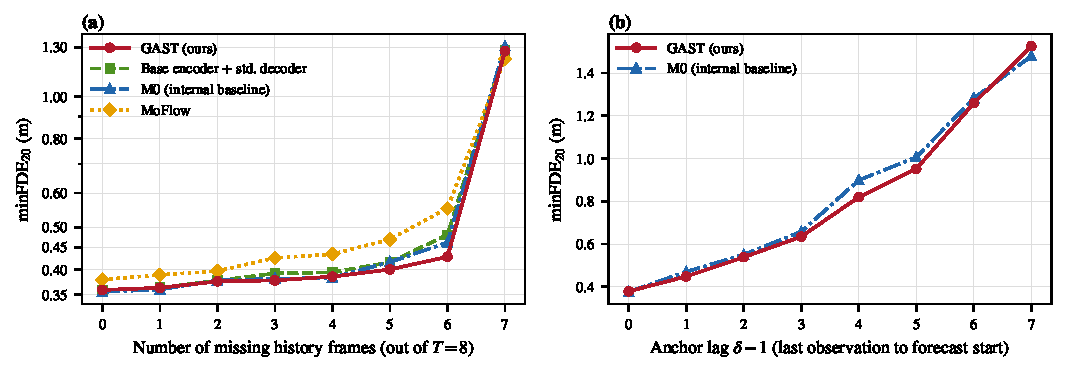
\includegraphics[width=\textwidth]{figures/degradation.pdf}
\caption{Degradation with respect to evidence loss (macro average over five scenes). (a)~$\mathrm{minFDE}_{20}$ as a function of the number of missing history frames, on a logarithmic scale; the dashed segment at seven frames reflects the qualitative change of regime in which a single observation remains. (b)~$\mathrm{minFDE}_{20}$ as a function of anchor lag, i.e.\ the number of steps between the last observation and the forecast origin. GAST's curve is flatter than the external baselines' at intermediate lags.}
\label{fig:degrad}
\end{figure*}

\subsection{Terminal missingness and anchor lag}
\label{sec:lag}

We report the same comparison along the two axes that the missing count confounds. Terminal missingness separates samples whose gap reaches the forecast origin from those whose gap ends earlier, and anchor lag counts the steps between the last observation and the origin. Among the external baselines, these diagnostics are available for SocialLSTM; MoFlow's evaluator emits only the missing-count axis.

The terminal group is the harder one for every method, and the gap between the groups is informative: relative to the non-terminal group, terminal-gap samples cost SocialLSTM $+75.0\%$ in $\mathrm{minFDE}_{20}$ (0.4547 to 0.7956), against $+61.4\%$ for GAST (0.3787 to 0.6112). GAST is 16.7\% better than SocialLSTM on the non-terminal group and 23.2\% better on the terminal group, so the relative advantage does not shrink where the anchor machinery is most exposed; this is the condition that the anchor state and the progress-conditioned skeleton were designed for.

Along anchor lag, GAST is better than SocialLSTM at every lag from 0 to 7, with the largest gaps at lags 3 and 4 ($-28.9\%$ and $-35.2\%$) and the smallest at the extreme lag 7 ($-7.4\%$), the regime in which only the first frame of the window is observed and the anchor is eight steps old. The shrinking margin at the extreme lag is the same phenomenon as the seven-missing bucket: beyond a certain evidence age, the estimate of the anchor velocity is dominated by noise, and a prior-driven forecast can approach an evidence-driven one. It suggests that the reliability decay should eventually saturate rather than continue to favour a very old state, which we leave to future work.

\subsection{Coverage versus ranking}
\label{sec:coverage}

Table~\ref{tab:top1} reports the top-1 diagnostics. GAST's $\mathrm{ADE@1}$/$\mathrm{FDE@1}$ are 0.9807/1.7887~m. Its $\mathrm{ADE@1}$ is statistically indistinguishable from MoFlow's (0.9814) and its $\mathrm{FDE@1}$ is 3.4\% worse than MoFlow's (1.7296), while its best-of-20 metrics are the best in the comparison and 7.6\% better than MoFlow's on the macro average. The dissociation between coverage and ranking is therefore mild relative to the strongest external baseline, but it is systematic: the top-1 margin narrows or reverses on scenes where the best-of-20 margin is large.

Our working hypothesis is that the goal-conditioned decoder, trained with an explicit diversity margin on endpoints and with trajectory-level mode labels, spreads the mode set and assigns probability mass more evenly, which improves coverage and simultaneously reduces the mass on the single best mode. This is a hypothesis about a mechanism, not a demonstrated causal explanation; we report it as an open problem, since a forecaster that is deployed behind a planner is usually consumed through its highest-probability mode.

\begin{table}[t]
\centering
\footnotesize
\setlength{\tabcolsep}{4.2pt}
\caption{Top-1 diagnostics (macro average, metres). $\mathrm{ADE@1}$/$\mathrm{FDE@1}$ use the highest-probability mode. Methods without mode probabilities are omitted.}
\label{tab:top1}
\begin{tabular}{@{}lcc@{}}
\toprule
Method & $\mathrm{ADE@1}$ & $\mathrm{FDE@1}$ \\
\midrule
MoFlow & \textbf{0.9814} & \textbf{1.7296} \\
GAST & 0.9807 & 1.7887 \\
SocialLSTM & 1.3278 & 2.1865 \\
\bottomrule
\end{tabular}
\end{table}

\subsection{Reproducibility}
\label{sec:repro}

The protocol, the Mixed adapter, the training runner, the evaluator and the model configuration are released as a single repository. Every run writes a manifest containing the git revision, the resolved configuration, the data files consumed, the checkpoint rule and the environment (Python, PyTorch and CUDA versions). Evaluation emits a JSON file with per-sample diagnostics for each of the five stratification axes, from which all tables in this paper are generated by script rather than transcribed by hand. The Laplace likelihood has two numerically equivalent implementations, one of which is vectorised; an equivalence gate verifies that their gradients agree to machine precision, and the implementation used by each run is recorded in its manifest.
